\documentclass[
	landscape,
	twocolumn,
	classe=$2^{de}$,
	exercices=Activité\space Chapitre\space 2
]{exercice}

\usepackage{tcolorbox}

\title{Union et intersection d'intervalles}
\author{}
\date{}

\newcommand{\intervalle}[4]{\left#1 #2;#3\right#4}

\setlength{\columnsep}{1cm}
\begin{document}

\newcommand{\Activite}{
	\maketitle

	\begin{tcolorbox}
		L'intersection de ces deux intervalles est l'ensemble des nombres qui sont dans l'un ET dans l'autre.

		L'union de ces deux intervalles est l'ensemble des nombres qui sont dans l'un OU dans l'autre.
	\end{tcolorbox}

	\begin{enumerate}
		\item Sur la droite ci-dessous, représenter l'intervalle $\intervalle{[}{2}{6}{]}$ en {\color{red}rouge}, et l'intervalle $\intervalle{[}{3}{8}{]}$ en {\color{blue}bleu} :
		      \begin{center}
			      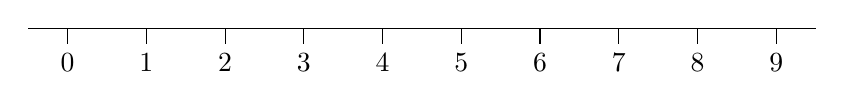
\begin{tikzpicture}
				      \draw[\myArrow] (-0.5,0) -- (9.5,0);
				      \foreach \x in {0,...,9} {
						      \draw (\x,0) -- ++(0,-0.2) node[below] {$\x$};
					      }
				      \ifdefined\makeCorrection
					      \foreach \x in {2.25,2.5,...,5.75} {
							      \draw[red] (\x,0) ++(0.15,0.15) -- ++(-0.3,-0.3);
						      }
					      \draw[red] (2.1,0.3) -- ++(-0.1,0) -- ++(0,-0.6) -- ++(0.1,0);
					      \draw[red] (5.9,0.3) -- ++(0.1,0) -- ++(0,-0.6) -- ++(-0.1,0);
					      \foreach \x in {3.25,3.5,...,7.75} {
							      \draw[blue] (\x,0) ++(-0.15,0.15) -- ++(0.3,-0.3);
						      }
					      \draw[blue] (3.1,0.3) -- ++(-0.1,0) -- ++(0,-0.6) -- ++(0.1,0);
					      \draw[blue] (7.9,0.3) -- ++(0.1,0) -- ++(0,-0.6) -- ++(-0.1,0);
				      \fi
			      \end{tikzpicture}
		      \end{center}
		\item Comment peut-on voir l'intersection des deux intervalles sur la droite ? \correction{Ce sont les points où \textbf{les deux} couleurs apparaissent.}
		\item Et l'union ? \correction{Ce sont les points où \textbf{au moins une des deux} couleurs apparaissent.}
		\item Écrire alors l'intersection et l'union de ces deux intervalles : \correction{intersection: $[3 ; 6]$, union : $[2 ; 8]$}.
		\item \newcommand{\itemSpacing}{0.3em}
		      Pour chacun des cas suivants, écrire l'union et l'intersection de $I$ et de $J$.
		      \begin{multicols}{2}
			      \begin{enumerate}
				      \item $I = \intervalle{[}{2}{6}{]}$ et $J = \intervalle{[}{3}{5}{]}$
				            \vspace{\itemSpacing}
				      \item $I =  \intervalle{]}{-∞}{-\frac{5}{2}}{[}$ et $J = \intervalle{]}{0}{-\frac{1}{4}}{[}$
				            \vspace{\itemSpacing}
				      \item $I =  \intervalle{]}{-∞}{\frac{5}{2}}{[}$ et $J = \intervalle{]}{-∞}{0}{[}$
				            \vspace{\itemSpacing}
				      \item $I =  \intervalle{]}{-∞}{1}{[}$ et $J = \intervalle{[}{-2}{+∞}{[}$
				            \vspace{\itemSpacing}
				      \item $I =  \intervalle{]}{\frac{1}{2}}{\frac{5}{4}}{]}$ et $J = \intervalle{[}{-\frac{1}{5}}{+∞}{[}$
				      \item $I =  \intervalle{]}{-5}{-1}{]}$ et $J = \intervalle{[}{3}{15}{]}$
			      \end{enumerate}
		      \end{multicols}
	\end{enumerate}
}

\Activite

\newpage
\Activite

\end{document}